\chapter{Lorentz Transformationen}
\label{sec:LorentzTransformationen}

I kapitel \ref{sec:GalileiTransformationen} omtalte vi de Galileiske koordinat transformations ligninger se (\ref{eq:Gx} - \ref{eq:Gt} i kapitel \ref{sec:GalileiTransformationen}). Disse transformationer\index{transformation} relatere koordinatet 
\begin{equation}
	\notag (x,y,z,t) ~\mathrm{i}~S \mapsto (x',y',z',t') ~\mathrm{i}~ S'
\end{equation}
Her er en af foruds�tningerne at det andet system $S'$ bev�ger sig med konstant fart $u$ relativt til systemet $S$ i positiv retning langs den f�lles $x-x'$ akse. Denne transformation antager ogs� at tidsskalaen er den samme i for de to systemer, hvilket fremg�r af ligning (\ref{eq:Gt}) i kapitel \ref{sec:GalileiTransformationen}. Som vi tidligere har vist g�lder Galilei transformationen\index{transformation!Galilei transformation} kun for gr�nseomr�det for $u$ g�ende mod nul.
Vi er derfor nu klar til at udlede en mere generel transformation som er konsistent med relativitets princippet\index{relativitets princippet}. Denne mere generelle transformation har f�et navnet \emph{Lorentz transformationen}\index{transformation!Lorentz transformation}.
Vores f�rste sp�rgsm�l er f�lgende:
\begin{quote}
	``\emph{N�r en begivenhed finder sted i punktet (x,y,z) til tiden t, som det observeres i systemet S, hvad er da koordinaterne (x',y',z') og tiden t' af begivenheden som den observeres i systemet S' som bev�ger sig relativt til S med konstant hastighed u og i positiv x-retning.}''
\end{quote}

For at udlede denne koordinat kransformation, refererer vi igen til figuren fra kapitel \ref{sec:GalileiTransformationen}. Som f�r, antager vi at de to systemers nulpunkter er sammenfaldende til tiden $t = 0 = t'$. Derfor er afstanden i $S$ fra $O$ til $O'$ til tiden $t$ stadig $ut$.

\begin{figure}
	\centering
		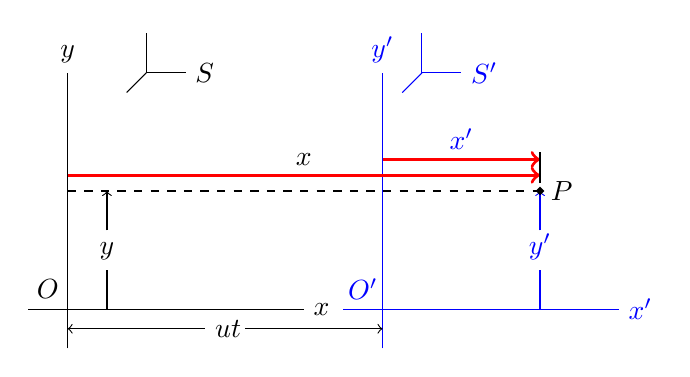
\begin{tikzpicture}
			% Tegn System 1
			\draw[black] (-.5,0) -- (3,0) node[right] {$x$};
			\draw[black] (0,-.5) -- (0,3) node[above] {$y$};
			\node[black] at (-0.25,0.25) {$O$};
			\draw[black] (1,3) --(1,3.5);
			\draw[black] (1,3) --(1.5,3) node[right] {$S$};
			\draw[black] (1,3) --(.75,2.75);
			
			% Tegn system 2
			\draw[blue] (3.5,0) -- (7,0) node[right] {$x'$};
			\draw[blue] (4,-.5) -- (4,3) node[above] {$y'$};
			\node[blue] at (3.75, 0.25) {$O'$};
			\draw[blue] (4.5,3) --(4.5,3.5);
			\draw[blue] (4.5,3) --(5,3) node[right] {$S'$};
			\draw[blue] (4.5,3) --(4.25,2.75);
			
			\draw[black, dashed] (0,1.5) -- (6,1.5);
			\draw[very thick, red, ->] (0,1.7) -- (6,1.7);
			\node[black,above] at ( 3,1.7) {$x$};
			\draw[very thick, red, ->] (4,1.9) -- (6,1.9);
			\node[blue,above] at (5,1.9) {$x'$};
			\draw[black, <-] (0,-.25) -- (1.75,-.25) node[right] {$ut$};
			\draw[black, ->] (2.25,-.25) -- (4,-.25);
			\draw[black] (0.5,0)  -- (0.5,0.5) node[above] {$y$};
			\draw[black, ->] (0.5,1) -- (0.5,1.5);
			\draw[blue] (6,0) -- (6,.5) node[above] {$y'$};
			\draw[blue, ->] (6,1) -- (6,1.5);
			\draw[black] (6,1.6) -- (6,2);
			\draw[very thick,black] (6,1.5) circle (.25mm) node[right] {$P$};
		\end{tikzpicture}
\end{figure}

Koordinatet $x'$ er en \emph{rigtig l�ngde} i $S'$, hvilket betyder at i systemet $S$ vil den v�re forkortet med en faktor:
\begin{equation}
	\notag\frac{1}{\gamma} = \sqrt{1-\tfrac{u^{2}}{c^{2}}}
\end{equation}
Som vi tidligere har vist om l�ngdeforkortning\index{l�ngdeforkortning}. Derfor vil afstanden $x$ fra $O$ til $P$, som den ses fra $S$ ikke blot v�re $x = x' + ut$, som vi kender fra Galilei transformationen\index{transformation!Galilei transformation} men derimod:
\begin{equation}\label{eq:L1}
	 x = ut + x'\cdot \sqrt{1-\frac{u^2}{\c^2}}
\end{equation}
L�ser vi nu denne ligning for $x'$ , finder vi frem til f�lgende:
\begin{equation}
	\tag{L.1}\label{eq:L2} x' = \frac{x-ut}{\sqrt{1-\frac{u^2}{\c^2}}} 
\end{equation}
Dette er den ene del af Lorentz transformationen\index{transformation!Lorentz transformation}. Den anden del af transformationen er den ligning som giver os $t'$ udtrykt ved $x$ og $t$. For at finde frem til denne ligning, skal vi noterer os at det relativistiske princip\index{relativitets princippet} kr�ver at \emph{formen} af transformationen fra $S$ til $S'$ skal v�re identisk med transformationen fra $S'$ til $S$. Den eneste forskel er at vi �ndre et fortegn i forhold til den relative hastigheds komponent $u$. Dermed kan ligning (\ref{eq:L1}) omskrives til
\begin{equation}\label{eq:L3}
	x' = -ut'+x\cdot\sqrt{1-\frac{u^2}{\c^2}}
\end{equation}
Vi kan nu s�tte ligning (\ref{eq:L2}) og (\ref{eq:L3}) lig med hinanden for at eliminere $x'$. Dette giver os en ligning for $t'$ udtrykt ved $x$ og $t$. Dette giver:
\begin{equation}
	\tag{L.2}\label{eq:L4} t' = \frac{t-\frac{ux}{c^2}}{\sqrt{1-\frac{u^2}{c^2}}}
\end{equation}
Som vi tidligere har omtalt s� er l�ngder m�lt vinkelret p� bev�gelsesretningen ikke p�virket af bev�gelsen, hvilket betyder at $y' = y$ og $z' = z$.

Samler vi nu alle udtrykkene sammen kan vi se at Lorentz transformatioenen\index{transformation!Lorentz transformation} best�r af f�lgende fire ligninger:
\begin{align}
	\label{eq:Lx}\tag{L.1} x' &= \frac{x-ut}{\sqrt{1-\frac{u^2}{\c^2}}} = \gamma\cdot(x-ut)\\
	\label{eq:Ly}\tag{L.2} y' &= y\\
	\label{eq:Lz}\tag{L.3} z' &= z\\
	\label{eq:Lt}\tag{L.4}  t' &= \frac{t-\frac{ux}{c^2}}{\sqrt{1-\frac{u^2}{c^2}}} = \gamma\cdot(t-\frac{ux}{c^2})
\end{align}
Dette s�t af ligninger er den generelle transformations beskrivelse mellem to initialsystemer i relativitetsteorien\index{relativitetsteorien}. Hvorfor vi herefter ikke l�ngere vil anvende Galilei transformationerne\index{transformation!Galilei transformation}, da disse som tidligere omtalt er begr�nsede til tilf�ldet hvor hastigheden $u$ g�r mod nul. 

\emph{\small Dette afsnit er baseret p� \cite{YF2005, Adams1997}.}